%%%%%%%%%%%%%%%%%%%%%%%%%%%%%%%%%%%%%%%%%
% Friggeri Resume/CV
% XeLaTeX Template
% Version 1.0 (5/5/13)
%
% This template has been downloaded from:
% http://www.LaTeXTemplates.com
%
% Original author:
% Adrien Friggeri (adrien@friggeri.net)
% https://github.com/afriggeri/CV
%
% License:
% CC BY-NC-SA 3.0 (http://creativecommons.org/licenses/by-nc-sa/3.0/)
%
% Important notes !!! : 
% Use texshop for better editor and this template needs to be compiled with XeLaTeX and the bibliography, if used,
% needs to be compiled with bibtex with biber backend.
%
%%%%%%%%%%%%%%%%%%%%%%%%%%%%%%%%%%%%%%%%%

\documentclass[]{friggeri-cv} % Add 'print' as an option into the square bracket to remove colors from this template for printing

\addbibresource{cv-dhoto.bib} % Specify the bibliography file to include publications
\usepackage[style=verbose,maxnames=99,sorting=ydnt,backend=biber]{biblatex}

\usepackage{fancyhdr}
\usepackage{lastpage}
 
\pagestyle{fancy}
\fancyhf{}
 
\rfoot{CV-Dhoto - Page \thepage \hspace{1pt} of \pageref{LastPage}}

\usepackage{wrapfig}
\usepackage[super]{nth}

\usepackage{lipsum}
%------------
\usepackage{enumitem}
\renewenvironment{entrylist}{%
  \begin{itemize}[leftmargin=1in]%[leftmargin=*,align=left,itemindent=-\dimexpr\labelwidth+\labelindent+\labelsep\relax]
}{%
  \end{itemize}
}
\renewcommand{\bfseries}{\headingfont\color{headercolor}}
\renewcommand{\entry}[4]{%
  \item[#1]
    \textbf{#2}%
    \hfill%
    {\footnotesize\addfontfeature{Color=lightgray} #3}\\%
    #4\vspace{\parsep}%
  }
%-------


\begin{document}

\header{Sritrusta}{ Sukaridhoto}{Assistant Professor, Researcher and Guitarist} % Your name and current job title/field

%----------------------------------------------------------------------------------------
%	SIDEBAR SECTION
%----------------------------------------------------------------------------------------

\begin{aside} % In the aside, each new line forces a line break
\section{contact}
\textbf{Politeknik Elektronika Negeri Surabaya}
Gedung Pascasarjana \nth{9} Floor, Room: PS09.03
Jl. Raya ITS Surabaya
~
Office:+62 (31) 5947280 ext:7902
Mobile:+62 823 6666 6379
~
\href{mailto:dhoto@pens.ac.id}{dhoto@pens.ac.id}
\href{http://dhoto.lecturer.pens.ac.id/}{Dhoto's Homepage}
\href{https://scholar.google.co.id/citations?user=M6sGfNQAAAAJ&hl=en&oi=ao}{Google Scholar}
\href{https://www.scopus.com/authid/detail.uri?authorId=35100882700}{Scopus-ID}
\href{http://facebook.com/iseng4h}{fb://iseng4h}


\section{languages}
Indonesian (native)
English \& Japanese 


\section{research interests}
{\color{red} $\varheartsuit$} Computer Networks,
Embedded System, Multimedia \& Internet of Things
\end{aside}

%----------------------------------------------------------------------------------------
%	MAIN SECTION
%----------------------------------------------------------------------------------------

\section{biography}

\begin{wrapfigure}[10]{l}{1.5in}
	\vspace{-10pt}
	\begin{center}
    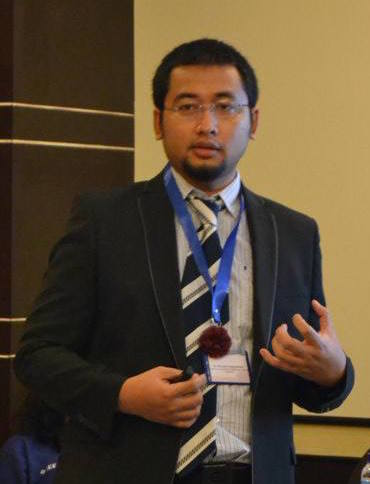
\includegraphics[width=0.2\textwidth]{dhoto-jas.jpg}
    \end{center}
    
\end{wrapfigure}
Received the B.E. degree in electrical engineering, computer science program from Sepuluh Nopember Institute of Technology, Indonesia, in 2002 and the Ph.D. degree in Communication Networks Engineering from Okayama University, Japan, in 2013. He joined at Politeknik Elektronika Negeri Surabaya, Indonesia, as a lecturer in 2002. He stayed at Tohoku University, Japan, in 2004, as a visiting researcher. From 2017, He become Head of Human Centric Multimedia Lab. His research interests include computer networks, embedded system, multimedia and Internet of Things. He has received several academic awards, best paper awards and IEEE Young Researcher Award in 2009. He is a member of IEEE.



\section{education}

\begin{entrylist}
%------------------------------------------------

\entry
{2009--2013}
{Doctor {\normalfont of Philosophy}}
{Okayama University, Japan}
{\emph{Engineering} \\ 
Dissertation: "A Study of Performance Improvement Methods for Real-Time Applications in Wireless Mesh Networks" \\
Supervised by Prof. Nobuo Funabiki, Prof. M. Hata and Prof. Toru Nakanishi}

%------------------------------------------------
\entry
{1997--2002}
{Bachelor {\normalfont of Engineering}}
{Institut Teknologi Sepuluh Nopember, Indonesia}
{Electrical Engineering - Computer Science\\
Thesis: “Implementation of IPv6 in Institute Technology Sepuluh November of Surabaya” 
\\Supervised by Dr. Surya Sumpeno and Dr. Supeno Mardi
}

%------------------------------------------------
\end{entrylist}

%----------------------------------------------------------------------------------------
%	WORK EXPERIENCE SECTION
%----------------------------------------------------------------------------------------

\section{work experience}

\begin{entrylist}
%------------------------------------------------
\entry
{2002-Now}
{Politeknik Elektronika Negeri Surabaya}
{Surabaya, Indonesia}
{\emph{Assistant Professor \& Head of Lab} \\
Department of Multimedia Creative Technology, 
\begin{itemize}
\item Teaching : Data Communication and Computer Networks
\item Supervision of Diploma students
\end{itemize}
Graduate School of Information Technology, 
\begin{itemize}
\item Teaching : Advanced Computer Networks and Internet of Things
\item Supervision of Master students
\end{itemize}
Head of Human Centric Multimedia Lab
}

%------------------------------------------------
%Masih berlangsung
\entry
{2019}
{Dinas Kependudukan dan Catatan Sipil}
{Surabaya, Indonesia}
{\emph{Big Data Infrastructur Consultant}}

\entry
{2017, 2018}
{Bank Jatim}
{Surabaya, Indonesia}
{\emph{IT Consultant}}



\entry
{2015-now}
{UGT Sidogiri - USAT}
{Pasuruan, Indonesia}
{\emph{Internet Service Provider Consultant}}

%------------------------------------------------
%Sudah selesai

\entry
{2017, 2018}
{PT. Eyro Digital Technology}
{Surabaya, Indonesia}
{\emph{IoT, Big Data architecture Consultant}}

\entry
{2016}
{Dinas Komunikasi dan Informatika}
{Surabaya, Indonesia}
{\emph{Network Security Consultant}}


%------------------------------------------------


\end{entrylist}

%----------------------------------------------------------------------------------------

\section{Skill}

Research and academic experiences with the field of Internet of Things, Computer Networks, Embedded System and Multimedia. Computer Programming and networking management skills with several programming languages for several projects such as hardware integration, web, Big Data analytic using Machine Learning, and Artificial Intelligence. Managerial skill as project manager and head of laboratory. 

%----------------------------------------------------------------------------------------

\section{signature}

The fully truth of the details are guaranteed. 
With strong sense of responsibility, hands on management and communication skills. 
Strong loyalty and self-motivation. 
\\
\\ 
regards, 
\\ 
\\
\\
\\
\textbf{Sritrusta Sukaridhoto, ST. Ph.D.} 


\end{document}